\documentclass{article}

\usepackage{tabularx}
\usepackage{booktabs}
\usepackage{tikz}

\title{Problem Statement and Goals\\\progname}

\author{\authname}

\date{}

\input{../Comments}
%% Common Parts

\newcommand{\progname}{MTOBridge} % PUT YOUR PROGRAM NAME HERE
\newcommand{\authname}{Team 15, Alpha Software Solutions
\\ Badawy, Adham
\\ Yazdinia, Pedram
\\ Jandric, David
\\ Vakili, Farzad
\\ Vezina, Victor
\\ Chiu, Darren} % AUTHOR NAMES                  

\usepackage{hyperref}
    \hypersetup{colorlinks=true, linkcolor=blue, citecolor=blue, filecolor=blue,
                urlcolor=blue, unicode=false}
    \urlstyle{same}


\begin{document}

\maketitle

\begin{table}[hp]
\caption{Revision History} \label{TblRevisionHistory}
\begin{tabularx}{\textwidth}{llX}
\toprule
\textbf{Date} & \textbf{Developer(s)} & \textbf{Change}\\
\midrule
9/22/2022 & Pedram Yazdinida & First Draft\\

\bottomrule
\end{tabularx}
\end{table}

\section{Problem Statement}

The approximate equations included in the Canadian Highway Bridge Design Code (CHBDC) (CSA S6-19) typically feature conservatism and add excessive costs. Although such extra costs are acceptable for designing new bridges, they may lead to unnecessary load restrictions or retrofitting of existing bridges. Using refined methods of analysis to precisely determine the load carrying capacity of bridge members would allow bridge engineers to make well-informed decisions on bridge repair and load posting.\\

This is an ongoing project in partnership with the Ontario Ministry of Transportation (MTO). The software engine application code has already been developed and validated by a Ph.D. student from the Department of Civil Engineering using MATLAB Editor. The developed MATLAB code is ready to be packaged with other software components (Interactive User Interface (UI), well-defined Input/Output (I/O), and standard bridge section Database). At the end of the project, we will work with the Capstone project team to produce a user manual and case study examples to facilitate the software implementation into evaluation/design practice.

\subsection{Problem}

\subsection{Inputs and Outputs}

%\wss{Characterize the problem in terms of ``high level'' inputs and outputs.  
%Use abstraction so that you can avoid details.}


\tikzset{every picture/.style={line width=0.75pt}} %set default line width to 0.75pt        

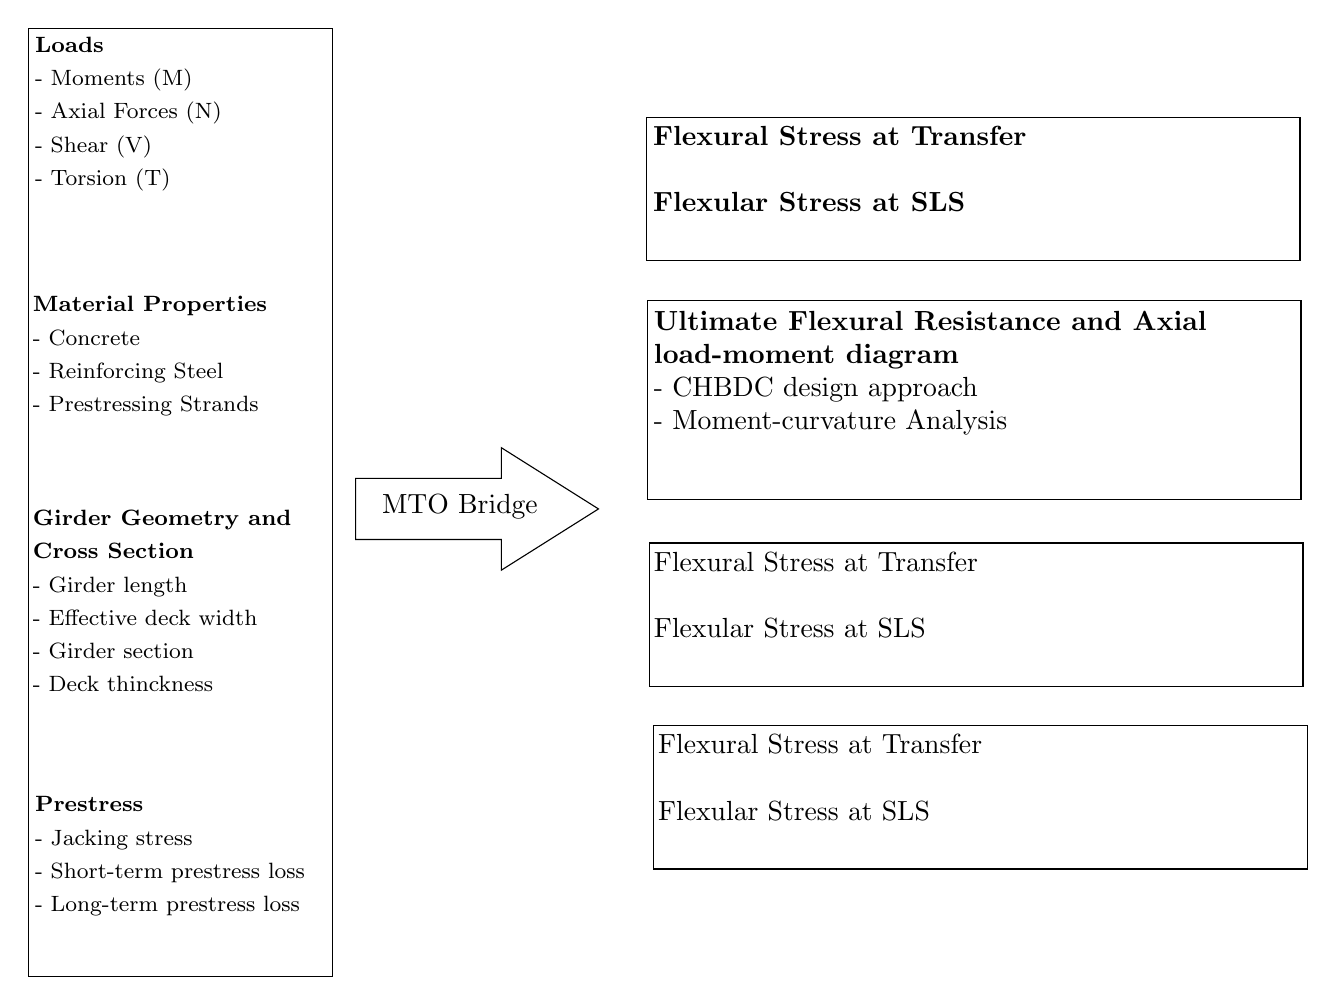
\begin{tikzpicture}[x=0.75pt,y=0.75pt,yscale=-1,xscale=1]
%uncomment if require: \path (0,554); %set diagram left start at 0, and has height of 554

%Shape: Rectangle [id:dp40713623006932687] 
\draw   (31.8,30.81) -- (178.55,30.81) -- (178.55,487.5) -- (31.8,487.5) -- cycle ;
%Right Arrow [id:dp022223857966380267] 
\draw   (189.55,247.66) -- (259.75,247.66) -- (259.75,232.91) -- (306.55,262.41) -- (259.75,291.91) -- (259.75,277.16) -- (189.55,277.16) -- cycle ;
%Shape: Rectangle [id:dp39774803382926405] 
\draw   (329.55,73.81) -- (644.55,73.81) -- (644.55,142.91) -- (329.55,142.91) -- cycle ;
%Shape: Rectangle [id:dp501499307053622] 
\draw   (330,161.81) -- (645,161.81) -- (645,257.91) -- (330,257.91) -- cycle ;
%Shape: Rectangle [id:dp9096357701279723] 
\draw   (331,278.81) -- (646,278.81) -- (646,347.91) -- (331,347.91) -- cycle ;
%Shape: Rectangle [id:dp47184812619999117] 
\draw   (333,366.81) -- (648,366.81) -- (648,435.91) -- (333,435.91) -- cycle ;

% Text Node
\draw (33.8,33.81) node [anchor=north west][inner sep=0.75pt]   [align=left] {\textbf{{\footnotesize Loads}}\\{\footnotesize - Moments (M) }\\{\footnotesize - Axial Forces (N)}\\{\footnotesize - Shear (V)}\\{\footnotesize - Torsion (T)}};
% Text Node
\draw (32.8,158.81) node [anchor=north west][inner sep=0.75pt]   [align=left] {\textbf{{\footnotesize Material Properties}}\\{\footnotesize - Concrete}\\{\footnotesize - Reinforcing Steel}\\{\footnotesize - Prestressing Strands}\\};
% Text Node
\draw (32.8,261.81) node [anchor=north west][inner sep=0.75pt]   [align=left] {\textbf{{\footnotesize Girder Geometry and }}\\\textbf{{\footnotesize Cross Section}}\\{\footnotesize - Girder length }\\{\footnotesize - Effective deck width}\\{\footnotesize - Girder section}\\{\footnotesize - Deck thinckness}};
% Text Node
\draw (33.8,399.81) node [anchor=north west][inner sep=0.75pt]   [align=left] {\textbf{{\footnotesize Prestress}}\\{\footnotesize - Jacking stress }\\{\footnotesize - Short-term prestress loss}\\{\footnotesize - Long-term prestress loss}};
% Text Node
\draw (201,254) node [anchor=north west][inner sep=0.75pt]   [align=left] {MTO Bridge};
% Text Node
\draw (331.55,76.81) node [anchor=north west][inner sep=0.75pt]   [align=left] {\textbf{Flexural Stress at Transfer }\\\\\textbf{Flexular Stress at SLS}};
% Text Node
\draw (332,165.81) node [anchor=north west][inner sep=0.75pt]   [align=left] {\textbf{Ultimate Flexural Resistance and Axial }\\\textbf{load-moment diagram}\\\mbox{-} CHBDC design approach \ \\\mbox{-} Moment-curvature Analysis };
% Text Node
\draw (332,281.81) node [anchor=north west][inner sep=0.75pt]   [align=left] {Flexural Stress at Transfer \\\\Flexular Stress at SLS};
% Text Node
\draw (334,369.81) node [anchor=north west][inner sep=0.75pt]   [align=left] {Flexural Stress at Transfer \\\\Flexular Stress at SLS};


\end{tikzpicture}
\begin{center}

\end{center}


\subsection{Stakeholders}

\begin{itemize}
  \item Ontario Ministry of Transport
  \item Department of Civil Engineering, McMaster
  \item Department of Software 
\end{itemize}
\subsection{Environment}
\begin{itemize}
  \item Compatible with the latest Windows 10 versions (20H1+)
  \item Fully operational offline 
  \item Requires C++ GNU compiler 
\end{itemize}
%\wss{Hardware and software}

\section{Goals}

\section{Stretch Goals}

\end{document}